\section{Chemical reactions}

\subsection{Reactions and CRN}
A reaction is just a set of reactants, a set of products, and a number $\kappa$ representing the speed of the reaction. Each reactant and product is some quantity of a species, these can be modelled as:  
\begin{minted}{haskell}
    type Reaction = Rxn of Map<species, float> * Map<species, float> * float
\end{minted}
Where the maps map a species to its concentration, the first map is the reactants, the second map is the products and the final float is $\kappa$.\\

Then \texttt{CRN} can be defined as the union of all the reactions, which can be stored in a reaction list:
\begin{minted}{haskell}
    type CRN = Reaction List
\end{minted}


\subsection{Simulation}
The ODE that we want to simulate describes the rate of change of concentration for a species \( S \) within a CRN. The equation is:
\[
\frac{d[S]}{dt} = \sum_{\forall \text{rxn} \in \text{CRN}} \kappa(\text{rxn}) \cdot \text{netChange}(S,\text{rxn}) \cdot \prod_{\forall R \in \text{reactants}(\text{rxn})} [R]^{m_{\text{rxn}}(R)}(t)
\]
This can be broken down into its components and translated to code, however, it can also be reformulated to use matrix operations, which in practice are highly optimized:

\[
\frac{d[S]}{dt} = N \cdot v(t)
\]
Where:
\begin{itemize}
    \item \( N \) is the net change matrix, and each element \( N_{ij} \) represents the scaled net change in species \( i \) due to reaction \( j \), including the reaction rate \( \kappa \). It is calculated using the following function:
\begin{minted}{haskell}
let genNetChangeMatrix (crn : CRN) (sl : species List) = 
    Matrix.ofJaggedList (List.foldBack (fun s st -> 
        genNetChangeList crn s :: st) sl [])
\end{minted}
Where \texttt{genNetChangeList} multiplies the reaction speed $c$ with the \texttt{netChange}:
\begin{minted}{haskell}
    let genNetChangeList (crn : CRN) (s : species) = 
        (List.foldBack (fun (Rxn(r,p,c)) st -> 
            c * (calcNetChange (Rxn(r,p,c)) s) :: st) crn [])
\end{minted}
and the \texttt{netChange} is calculated by:
\begin{minted}{haskell}
    let calcNetChange (Rxn(r, p, c)) (s: species) = 
        (getValue p s) - (getValue r s) 

\end{minted}

    \item \( v(t) \) is a vector where each component corresponds to the product of the concentrations of reactants raised to their stoichiometric coefficients for each reaction at time \( t \). This vector is computed by:
\begin{minted}{haskell}
let calcReactionProducts (state : State) (crn : CRN) = 
    vector (
        List.map (fun (Rxn(r, _, _)) ->
            Map.fold (fun s coeff prod -> 
                prod * (state |> Map.find s) ** coeff) 1.0 r
        ) crn
    )
\end{minted}
\end{itemize}

We wanted to further optimize the calculation of \(v(t)\), by using the logarithm to transform it into a dot-product, however, this led to problems due to the possibility of there being zeros.\\

Then a single step can be calculated by finding this derivative for all species:
\begin{minted}{haskell}
    let simulateStepMatrix state crn netChangeMatrix (sl : species List) timestep = 
        let change = calcDerivatives netChangeMatrix 
            (calcReactionProducts state crn) timestep
        List.fold (fun map (s,ds) -> 
            Map.add s ((getValue state s) + ds) map) 
                state (List.zip sl (List.ofArray (Vector.toArray change)))
\end{minted}
And the derivatives comes directly from the discussed formula:
\begin{minted}{haskell}
    let calcDerivatives netChangeMatrix reactionProduct timestep =
        timestep * (netChangeMatrix * reactionProduct) 
\end{minted}

Lastly, the infinite sequence of simulations can then be calculated using an \texttt{unfold}:
\begin{minted}{haskell}
    let simulateReationsMatrix (state : State) (crn : CRN) (timestep : float) = 
    let sl = Set.toList (Set.ofList (
            List.fold
                (fun sp (Rxn(r, p, c)) ->
                    Map.fold (fun keys k _ -> k :: keys) [] r
                    @ Map.fold (fun keys k _ -> k :: keys) [] p
                    @ sp)
                []
                crn
        ))
    let netChangeMatrix = genNetChangeMatrix crn sl

    Seq.unfold (fun st -> let nextState = 
        simulateStepMatrix st crn netChangeMatrix sl timestep
            Some(nextState,nextState)) state

\end{minted}

\subsection{Visualization}
Since this simulation results in a sequence of states, just like the interpreter from the prior section, we can use the visualization code from the interpreter to visualize the simulation. Here is an image of the gcd program where a is 32 and b is 12, and one of the Euler number calculator:

\begin{figure}[H]
    \centering
    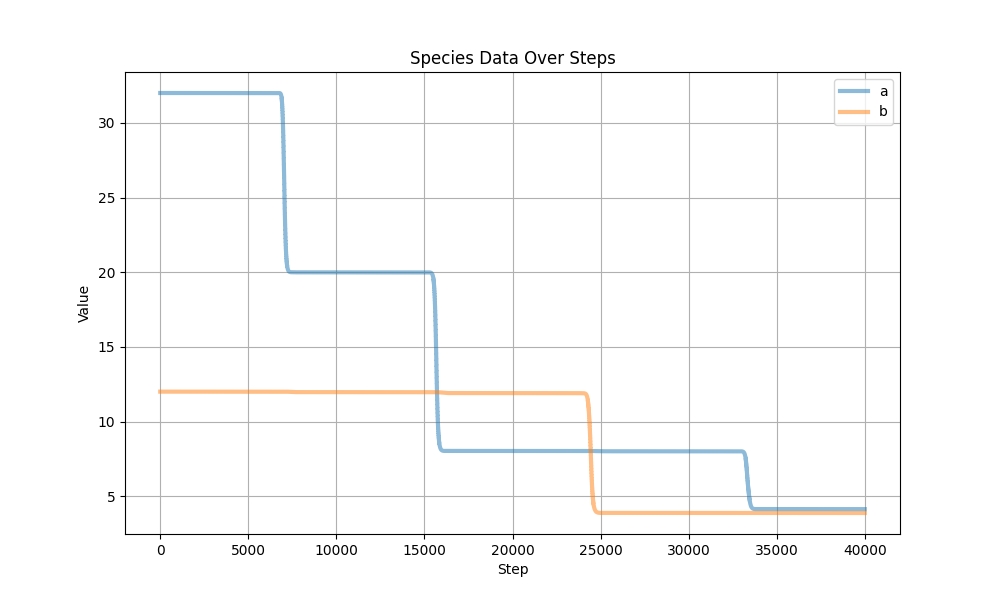
\includegraphics[scale=0.3]{report/figures/gcdplot.png}
    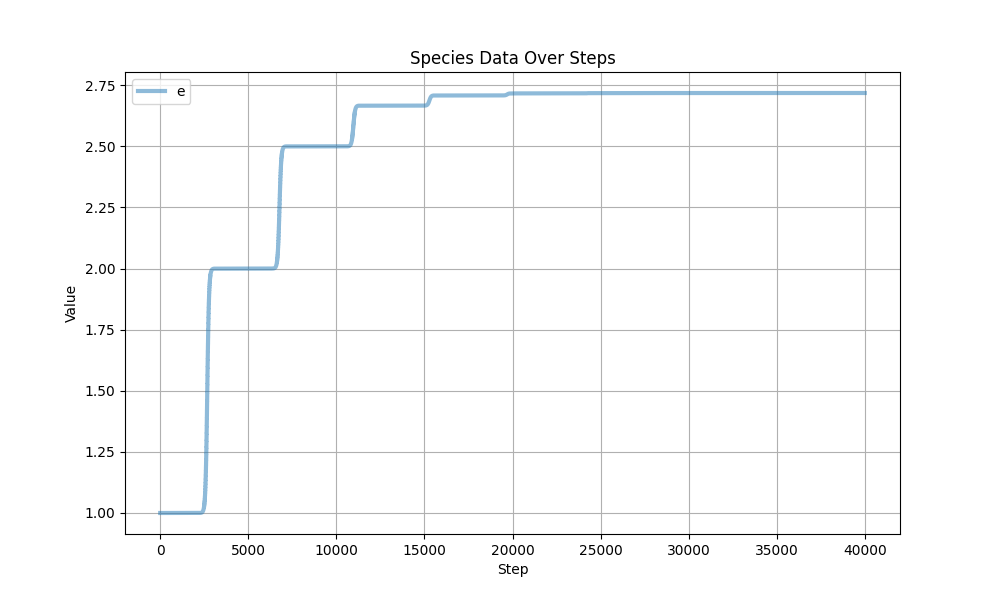
\includegraphics[scale=0.3]{report/figures/eulerplot.png}
\end{figure}
\subsection{Testing}
To test that the simulations work, simulations on the arithmetic components were tested in the same manner as in the previous section. Due to the slow convergence of the simulations, it is computationally intensive to test the larger programs. Therefore we did not make tests that compare the output from simulated programs to the calculated results. 

\subsection{Assessment}